\documentclass[10pt,english]{article}
\usepackage[T1]{fontenc}
\usepackage[utf8]{inputenc}
\usepackage{lmodern}
\usepackage{amsmath,amssymb,booktabs,graphicx}
\usepackage[main=english]{babel}
\usepackage[margin=0.72in]{geometry}
\usepackage{xcolor}
\usepackage[skins,breakable]{tcolorbox}
\usepackage{titlesec}
\usepackage{needspace}
\usepackage{microtype}
\usepackage{xurl}
\usepackage{hyperref}
\hypersetup{pdftitle={Probability-Valued Subset Sum: Certified Bounds and Learned Guidance},
  pdfauthor={Jonathan R. Landers},hidelinks}
\definecolor{paperink}{HTML}{26231F}
\definecolor{paperaccent}{HTML}{6E5943}
\definecolor{paperline}{HTML}{C8BCAD}
\definecolor{paperboxbg}{HTML}{F7F3EC}
\color{paperink}
\titleformat{\section}{\normalfont\large\bfseries\color{paperink}}{}{0pt}{\color{paperaccent}\rule{2pt}{1.05em}\hspace{7pt}}
\titlespacing*{\section}{0pt}{11pt}{5pt}
\tcbset{paperbox/.style={enhanced,breakable,colback=paperboxbg,colframe=paperline,
  boxrule=.45pt,arc=2mm,left=8pt,right=8pt,top=6pt,bottom=6pt,
  before skip=6pt,after skip=8pt},
  accentbox/.style={paperbox,borderline west={2pt}{0pt}{paperaccent}}}
\setlength{\parindent}{0pt}
\setlength{\parskip}{5pt plus 1pt minus 1pt}
\setlength{\emergencystretch}{3em}
\title{Probability-Valued Subset Sum:\\ Certified Bounds and Learned Guidance}
\author{Jonathan R. Landers}
\date{October 2026}
\begin{document}
\maketitle
\vspace{-1.5em}
\noindent\textcolor{paperaccent}{\footnotesize\textsc{Companion note III of III}}
\par\noindent\textcolor{paperaccent}{\rule{.11\linewidth}{1.5pt}}\textcolor{paperline}{\rule{.89\linewidth}{.45pt}}
\vspace{.4em}

\begin{tcolorbox}[accentbox]
\textbf{Abstract.} The first note asks when certified coverage can replace explicit search; the second finds no incremental exact subset-sum gain from the tested pairing method. This note changes the question: for fixed weights and a specified random target, what is the probability that some subset reaches it? Witnessed sums and sound exclusions give deterministic bounds on this probability. On \(50\) held-out \(16\)-item lists, the median lower and upper endpoints from simple rules were \(0.8\%\) and \(36.0\%\), while the median exact reachable-target fraction was \(24.2\%\). A learned classifier supplies useful statistical ranking but no per-instance certificate. The bounds and experiments suggest an approximate, costed coverage problem rather than a faster exact decision algorithm.
\end{tcolorbox}

\section{The probability requires a random experiment}
For fixed positive weights \(w=(w_1,\ldots,w_n)\) and target \(t\), the decision answer
\[
Y(w,t)=\mathbf{1}\!\left\{t=\sum_{i=1}^n x_iw_i
  \text{ for some }x\in\{0,1\}^n\right\}
\]
is exactly \(0\) or \(1\). To obtain a probability, let \(D\) be a finite target set, \(T\) a random target with distribution \(\mu\) supported on \(D\), and
\[
A(w)=\left\{\sum_{i=1}^n x_iw_i:x\in\{0,1\}^n\right\}.
\]
\begin{tcolorbox}[accentbox]
\[
q_\mu(w)=\Pr_{T\sim\mu}[Y(w,T)=1]
        =\sum_{t\in A(w)\cap D}\mu(t).
\]
\end{tcolorbox}
For a uniform target, \(q_\mu(w)=|A(w)\cap D|/|D|\). Thus the new outcome is the chance that a target drawn by a \emph{stated rule} is reachable. Changing \(D\) or \(\mu\) changes the question; the probability is not uncertainty about a fixed target.

\section{Bounds that remain correct for one list}
Let \(L\subseteq A(w)\cap D\) be distinct sums with explicit subset witnesses. For a positive modulus \(m\), let \(R_m(w)=\{a\bmod m:a\in A(w)\}\). Given a finite collection \(M\) of moduli, define
\[
U=D\cap\bigcap_{m\in M}\{t:t\bmod m\in R_m(w)\}.
\]
\begin{tcolorbox}[accentbox]
\textbf{Proposition 1 (Certified probability interval).}
For every \(w,D,\mu,L,M\) defined above,
\[
\mu(L)\le q_\mu(w)\le\mu(U),
\qquad \mu(B):=\sum_{t\in B}\mu(t).
\]
\end{tcolorbox}
\textit{Proof.} Every witnessed sum belongs to \(A(w)\), giving \(L\subseteq A(w)\cap D\). Every attainable sum has an attainable residue modulo every \(m\in M\), giving \(A(w)\cap D\subseteq U\). Monotonicity of probability mass proves both inequalities. \hfill\(\square\)

Repeated values give another cheap bound. If distinct weight value \(v_j\) occurs \(c_j\) times, at most \(c_j+1\) copies of that value can be chosen. Hence
\[
|A(w)|\le K(w):=\prod_j(c_j+1).
\]
For a uniform target on \(D\), combine the two upper bounds:
\begin{tcolorbox}[accentbox]
\[
\frac{|L|}{|D|}\le q_\mu(w)\le
\min\left\{\frac{|U|}{|D|},\,\frac{K(w)}{|D|},\,1\right\}.
\]
\end{tcolorbox}
The count \(K(w)\) is only an upper bound: different count vectors may have the same sum. Exact paired summaries can enlarge \(L\), but their distinct union must be counted, and their construction cost must be charged. More sound exclusions can shrink \(U\).

The interval certifies an additive-\(\varepsilon\) answer whenever its width is at most \(\varepsilon\). Exact \(q_\mu\) requires zero width. This is the probability analogue of the first note's costed coverage idea: bound quality matters together with the cost of producing it.

\section{A direct check of bound quality}
We reused the held-out \(n=16\) lists from the classifier experiment in note II. For each of \(50\) lists, the target set \(D\) was the integer middle \(40\%\) of the list's total sum, restricted to targets that passed the experiment's residue tests modulo \(8,10,16,32\). Conditional on that filter, targets were drawn uniformly from \(D\). The same residue tests therefore supply no further upper-bound reduction on this particular \(D\).

The lower bound used distinct sums from \(512\) randomly sampled subsets; the upper bound used \(K(w)/|D|\). We enumerated all attainable sums to measure the exact \(q_\mu(w)\) \emph{for evaluation only}. Each computed interval contained the exact value.

\begin{table}[h]
\centering
\caption{Medians across held-out \(n=16\) lists. Columns are separate medians, not one interval for a representative list.}
\small
\begin{tabular}{lrrrr}
\toprule
Family & Lists & Witness lower & Exact \(q_\mu\) & Count upper\\
\midrule
Independent weights & 26 & \(0.3\%\) & \(25.8\%\) & \(36.9\%\)\\
Repeated pairs & 24 & \(2.2\%\) & \(24.2\%\) & \(36.0\%\)\\
All lists & 50 & \(0.8\%\) & \(24.2\%\) & \(36.0\%\)\\
\bottomrule
\end{tabular}
\end{table}

\begin{figure}[h]
\centering
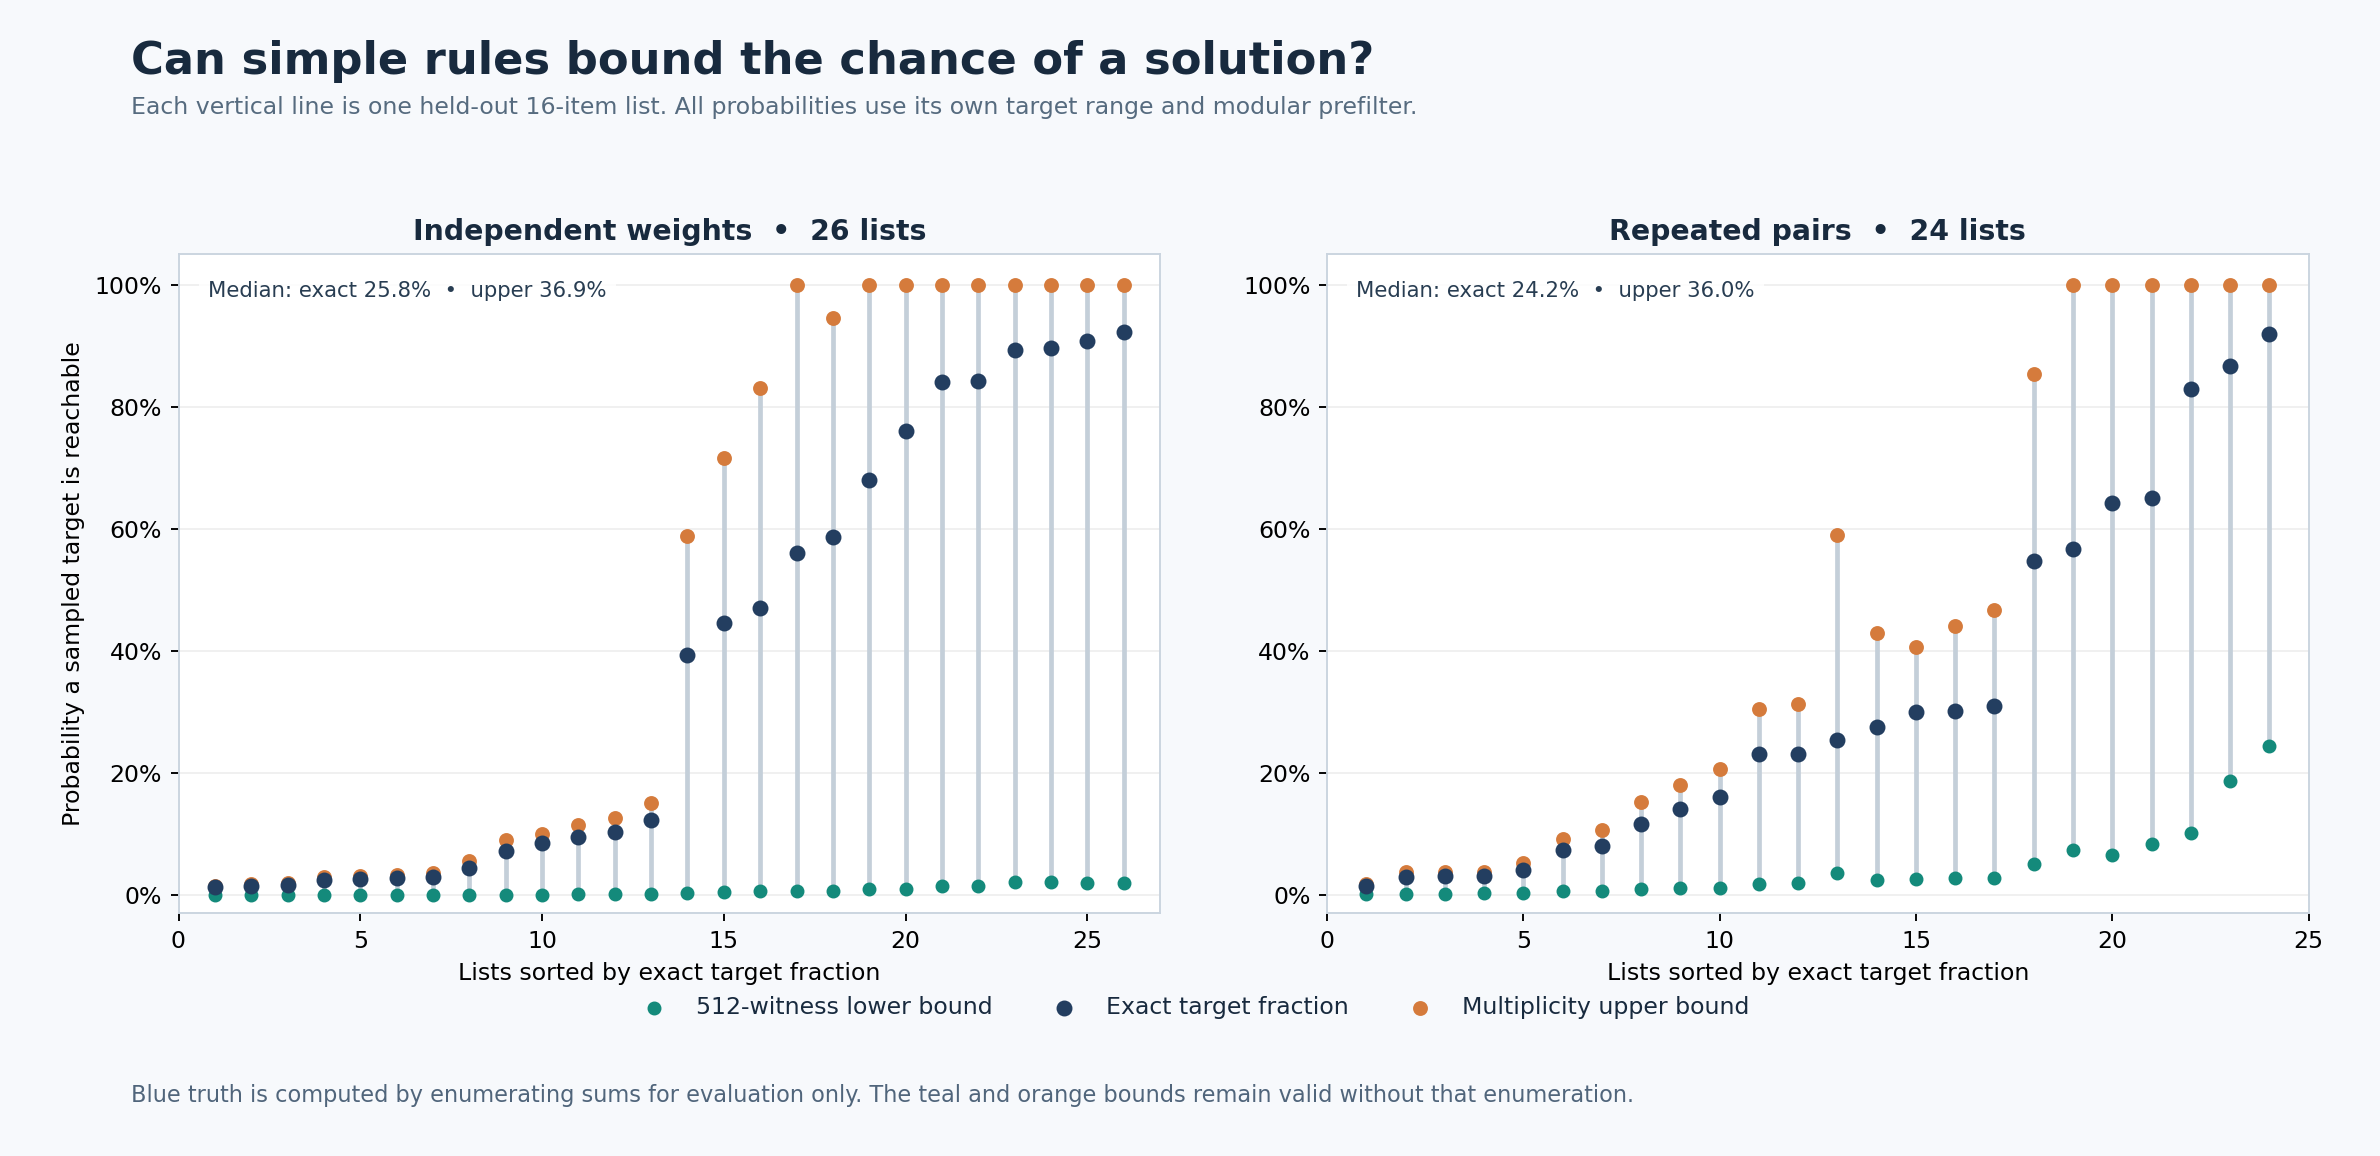
\includegraphics[width=.98\linewidth]{subset-sum/instance_probability_bounds.png}
\caption{Each vertical segment is a certified interval for one list; the dark point is its exact reachable-target fraction. The low-budget witness bound is often loose.}
\end{figure}

These bounds do not claim a runtime improvement. They show that counting possible selections can sometimes limit the probability without deciding each target, while a small witness budget leaves much of the mass unresolved.

\section{Statistical probabilities and learned guidance}
The classifier in note II outputs \(\widehat p(w,t)\). Since \(Y(w,t)\) is fixed once the full instance is known, \(\widehat p\) is best understood as an estimate of \(\Pr(Y=1\mid\phi(w,t))\) under a specified input distribution, where \(\phi\) is the model's lossy feature vector. It is distinct from the exact \(q_\mu(w)\) for one fixed list.

The held-out experiment drew four targets per independent list. Its \(229\) YES answers among \(720\) targets give an observed rate of \(31.8\%\) across the \(180\) held-out lists. A \(95\%\) bootstrap interval resampling whole lists is \(26.9\%\)--\(36.7\%\). Treating each list's four-target average as one bounded independent observation gives a wider Hoeffding \(95\%\) interval of \(21.7\%\)--\(41.9\%\) for the mean success rate across that test schedule. On \(240\) unseen \(n=24\) lists, the observed rate was \(25.0\%\) across \(960\) targets; the list-bootstrap interval was \(20.9\%\)--\(29.2\%\). These rates depend on the synthetic list and target generators.

For a \emph{fixed} list, \(m\) independent random targets with exact labels also give the standard sampling bound
\[
\Pr\{|\widehat q-q_\mu(w)|>\varepsilon\}\le 2e^{-2m\varepsilon^2}.
\]
The exact-label cost remains. Sampling uncertainty intervals are different from Proposition 1's deterministic bounds.

At the classifier threshold \(\widehat p\le1\%\), \(2\) of \(43\) held-out proposed NO answers were actually YES. The list-bootstrap interval for that conditional error fraction was \(0\%\)--\(10.7\%\); its zero lower endpoint does not certify zero future risk. A learned score can order which witnesses or certificates to seek, but cannot itself certify a NO decision.

\section{Next question}
The useful research target is a cheap sequence of witnessed sets \(L\) and sound supersets \(U\) whose mass gap closes quickly for a meaningful target distribution. One can measure bound width after a fixed budget, or total work to reach a chosen \(\varepsilon\), against direct exact enumeration and sampling with exact labels. The present results motivate this experiment; they do not show a new complexity bound or exact subset-sum speedup.

\vspace{.4em}
\noindent\textbf{Series and reproducibility.} Note I: \emph{Certified Coverage of Exponential Search Spaces}. Note II: \emph{Subset Sum as a Stress Test for Certified Coverage}. Scripts, figures, and held-out predictions: \url{https://github.com/jonland82/exponential-search-spaces}.
\end{document}
